\section{Introduction}

Evaluating frontier models is becoming more expensive as they become more sophisticated \citep{burden2024evaluating,openai2023gpt4}.
At the same time, with new models arriving in quick succession, and ever-present scope for data to leak from evaluations to training \citep{ganguli2023challenges}, the evaluation problem is a dynamic one: it requires ongoing, adaptive gathering of new evaluation data.

Active testing \citep{kossen2021active,kossen2022active} is an attractive solution to this problem.
Motivated by the observation that some labels are more informative than others about the behaviour of a target model, it involves carefully deciding which test inputs to acquire labels for.
The foundation for data acquisition is a surrogate model of the test-time label distribution, which is typically updated on the labels acquired during testing.
Making a data-acquisition decision requires making predictions with the surrogate model and often also the target model.
The computational cost of this process is often justifiable in light of high labelling costs, but it limits the scope of active testing's applicability.

In this work we show how active testing can be scaled up to large language models (LLMs), allowing us to more effectively evaluate them with limited labelling budgets.
We begin by highlighting three computational bottlenecks in the predominant approach to active testing: updating the surrogate model as labels are acquired, making predictions with the surrogate model, and making predictions with the target model.
The first of these is particularly important: it has traditionally involved repeatedly running gradient-based training on the acquired test data within an active-testing loop.


\begin{figure}[t]
    \centering
    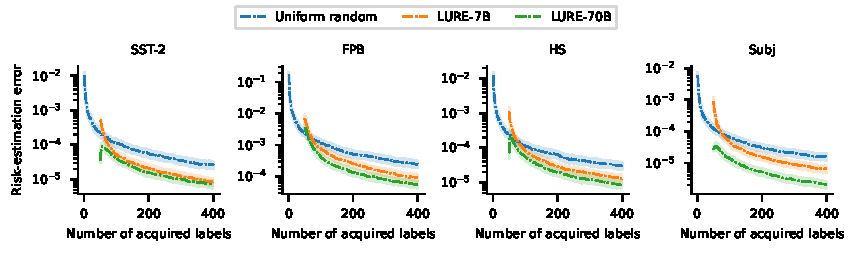
\includegraphics[width=\textwidth, trim={0 5pt 0 0}]{
        figures/pdf/70b_zeroshot_unif_lure.pdf
    }
    \caption{
        Our proposed active-testing approach enables low-error estimates of the risk (expected predictive loss) of a large language model (here the 70B version of Llama 2) on four text-classification problems (SST-2, FPB, HS and Subj) while only using a small label budget.
        We compare uniform-random testing against active testing (LURE), using either a 7B or 70B surrogate model with in-context learning to guide data acquisition.
    }
    \label{fig:70b_zeroshot_unif_lure}
    \vspace{-8pt}
\end{figure}


We then identify simple and surprisingly effective ways to address each of these key bottlenecks.
First, we strip back the training of the surrogate model to a single step of in-context learning \citep{brown2020language} on a small amount of initial test data, removing the need for repeated gradient-based training.
Second, we show it is possible to use a surrogate model that is smaller than the target model, reducing the cost of surrogate-model predictions.
Third, we show we can even forgo making any predictions with the target model, relying solely on the surrogate model for data acquisition.
Together these changes make active testing dramatically cheaper, enabling it to be scaled up to LLMs.

Empirically we find our approach can substantially improve over the common practice of acquiring data uniformly at random (\Cref{fig:70b_zeroshot_unif_lure}).
More specifically it can estimate the risk (expected predictive loss over test examples) of LLMs with an estimation error typically 25\% to 50\%---and sometimes up to 80\%---lower than that obtained through uniform-random data acquisition.
Our work therefore represents significant progress in accurately and dynamically evaluating LLMs, as well as in more generally increasing the scope for active testing to be used in practical settings.

To further improve the real-world applicability of active testing, we address the challenge of judging how well it is working on a given problem.
In research we can assess active testing by running it multiple times and comparing its risk estimates to a known true risk.
But practical deployment involves running active testing only once, without knowledge of the true risk, making it hard to gauge active-testing performance.
To help address this we derive a bootstrap estimator \citep{efron1979bootstrap} of the risk-estimation error.
In experiments we find our approximate 95\% confidence intervals contain the true risk-estimation error 88\% of the time, suggesting our estimator can be a useful diagnostic tool.